% ISM 2026 Paper
% Title: Configuration, Not Code: A Human-in-the-Loop LLM Architecture for Mapping
%        Heterogeneous Enterprise Systems to Canonical Digital Twin Models
% Target track: Reshaping future smart manufacturing: convergence of Industrial Metaverse,
%               Cyber-Physical Systems, and Digital Twins

\documentclass[3p,times,procedia]{elsarticle}
\flushbottom

\usepackage{ecrc}
\usepackage[bookmarks=false]{hyperref}
    \hypersetup{colorlinks,
      linkcolor=blue,
      citecolor=blue,
      urlcolor=blue}
\usepackage{amssymb}
\usepackage[figuresright]{rotating}
\usepackage{graphicx}
\usepackage{booktabs}

\volume{00}
\firstpage{1}
\journalname{Procedia Computer Science}
\runauth{K. Bohara et al.}
\jid{procs}

\begin{document}
\begin{frontmatter}

\dochead{8th International Conference on Industry of the Future and Smart Manufacturing}

\title{Configuration, Not Code: A Human-in-the-Loop LLM Architecture for Mapping Heterogeneous Enterprise Systems to Canonical Digital Twin Models}

\author[a]{Kshitiz Bohara\corref{cor1}}
\author[a]{Richard Reider}
\author[a]{Tobias Reggelin}
\author[a,b]{Sebastian Lang}

\address[a]{Institute for Engineering of Products and Systems, Otto-Von-Guericke-University Magdeburg,
GERMANY}
\address[b]{Fraunhofer Institute for Factory Operation and Automation IFF, Magdeburg, Germany}

\begin{abstract}
Manufacturing enterprises sit on decades of data locked in heterogeneous ERP and MES systems, yet building digital twins from this data today requires per-customer code, embedded consultants, and manual field mapping, excluding the SMEs who stand to gain the most. We present a human-in-the-loop architecture where an LLM reads raw enterprise API payloads, consults a curated catalog of target-schema field descriptions, and proposes field-level mappings as JSON configuration with calibrated confidence scores. A human reviews only the fields the model flags as uncertain, while high-confidence proposals are safe to auto-accept. A deterministic runtime engine consumes the configuration and assembles the digital twin with zero per-customer code. The architecture is vendor-agnostic: heterogeneous source systems map to any canonical information model (exemplified here by CMSD/ISO 22400). Across two LLM architectures, four API payload variants, and controlled RAG ablation, both models achieve 95--96\% aggregate mapping accuracy. The non-reasoning model matches the reasoning model within 1.4 percentage points while running 3$\times$ faster with lower token consumption. Extended statistical analysis ($n=20$, 640 runs) reveals that field ambiguity, predominantly in numeric fields within legacy payloads, is the fundamental bottleneck; target-side RAG provides zero statistically significant improvement (Mann--Whitney $U$, $p > 0.05$). The architecture, not the model, is the contribution.
\end{abstract}

\begin{keyword}
digital twin ; large language model ; human-in-the-loop ; CMSD ; smart manufacturing ; enterprise integration ; configuration-driven architecture ; canonical information model
\end{keyword}
\cortext[cor1]{Corresponding author. }
\end{frontmatter}
\email{kshitiz.bohara@ovgu.de}

% =============================================================================
% 1. INTRODUCTION
% =============================================================================
\section{Introduction}
\label{sec:intro}

Consider a mid-sized CNC machining supplier seeking to adopt digital twin technology for its own operations: simulating production schedule changes, tracking overall equipment effectiveness, and optimizing resource allocation across its shop floor. The simulation software expects data conforming to a vendor-neutral standard such as Core Manufacturing Simulation Data (CMSD). The supplier's data, however, is fractured across systems that were never designed to interoperate: static master data lives in an on-premise SAP ERP with German field names, while operational data sits in a legacy MES whose API returns opaque, undocumented field codes. Today, bridging this gap requires an embedded consultant who manually inspects each API response, maps every field to the target schema by hand, and hard-codes per-customer Python scripts. For the thousands of SMEs with limited IT staff and no in-house domain expertise, this cost is prohibitive, excluding them from digital twin adoption.

This scenario is the norm. Decades of structured factory data are locked inside heterogeneous ERP, MES, and SCADA systems, each using its own naming conventions for the same manufacturing concepts. The manual mapping approach is brittle to API changes and carries a per-customer cost structure that makes digital twins viable only for large enterprises.

Large Language Models offer a different path. An LLM can parse a raw API payload, understand a target schema expressed in plain language, and propose field-level mappings with self-assessed confidence scores. This inverts the architecture: instead of generating per-customer code, the LLM produces a JSON configuration that declaratively specifies every mapping and transformation. A human reviews only the proposals the model flags as uncertain. A deterministic runtime engine consumes the configuration and assembles the digital twin, with zero generated code. The mapping is a configuration artifact, not a software artifact.

This paper presents the architecture, implementation, and empirical evaluation of a system that realizes this vision. Our contributions are threefold:

\begin{itemize}
\item \textbf{Architecture.} A configuration-driven, human-in-the-loop architecture where an LLM proposes field mappings as JSON at design time, a deterministic engine assembles the twin at runtime, and a vendor-neutral canonical information model serves as the integration hub for heterogeneous enterprise APIs.
\item \textbf{Calibrated Human-in-the-Loop Workflow.} The LLM self-scores every mapping proposal, enabling targeted human review of only uncertain fields while high-confidence proposals are safe to auto-accept. Smart reanalysis re-evaluates only corrected fields.
\item \textbf{Empirical Validation.} A controlled evaluation across two LLM architectures, four API payload variants, and controlled RAG conditions, demonstrating that a non-reasoning model matches reasoning-model accuracy at lower cost, and that numeric field ambiguity in legacy payloads is the fundamental bottleneck for automated schema mapping.
\end{itemize}

% =============================================================================
% 2. RELATED WORK
% =============================================================================
\section{Related Work}
\label{sec:related}

The instantiation of digital twins from enterprise data sources spans a spectrum of architectural paradigms, ranging from rigid, hardcoded logic and bespoke factory modeling \cite{Jia2022From,Lugaresi2021Automated} to highly automated approaches utilizing rule-based mapping engines and template-driven code generation \cite{Lehner2025Model-driven,Schroeder2021A}. However, even within these automated Model Driven Engineering (MDE) paradigms, significant technical friction remains. An expert must still deeply understand both the source API structure and the target information model to manually author the foundational transformation rules before any automation can occur. Consequently, these pipelines are highly susceptible to schema drift; a minor API version update or the introduction of a heterogeneous ERP vendor often invalidates existing models, forcing manual recalibration of the mapping logic. Despite this persistent integration bottleneck, existing reference architectures for manufacturing digital twins \cite{inbook,ZVEI2015RAMI40,iso23247-1} frequently abstract away the upstream mapping problem entirely. The majority operate under the idealized assumption that enterprise data is already harmonized in the target format, leaving the critical challenge of dynamic semantic alignment unresolved \cite{Hildebrandt2024Data,Jeddoub2024Data}.

Schema mapping and ontology alignment have been studied extensively in the data integration community. Traditional approaches use rule-based matchers, dictionary-based string similarity measures, and heuristic structural matching across database schemas \cite{Halevy2005Why}. More recently, large language models have been applied to zero-shot and few-shot schema mapping tasks, demonstrating that LLMs can match fields across database schemas and knowledge graphs without task-specific training \cite{parciak2024schemamatchinglargelanguage}. In parallel, human-in-the-loop methods have been explored for interactive schema matching and entity resolution, where machine proposals are refined through human feedback \cite{10.14778/3352063.3352068}. Our work sits at the intersection of these two lines: we combine LLM-based mapping proposals with a calibrated confidence framework that directs human attention exclusively to uncertain proposals, an approach we argue is the right balance for industrial settings where mapping correctness directly impacts production decisions.

To anchor this AI-driven mapping process within a standardized industrial ontology, we utilize the CMSD standard. The standard defines a vendor-neutral information model for exchanging manufacturing simulation data across tools and organizations \cite{58196}. However, implementations have predominantly utilized CMSD as a static, file-based artifact (e.g., XML) for open-loop simulation tool interoperability \cite{26646,Zhao2024An}. Our implementation operationalizes CMSD as a dynamic runtime canonical hub for multi-source enterprise integration. In a significant departure from legacy file-exchange paradigms, our approach translates the static CMSD schema into strongly typed, executable models deployed as live, containerized microservices. Coupled with an LLM-driven field mapper, this architecture enables a single configuration-driven pipeline to continuously translate heterogeneous ERP and MES data streams into a live CMSD execution environment.

By automating the semantic mapping phase and virtualizing the target ontology, this framework directly addresses the systemic challenges facing smaller enterprises. Barriers to digital twin adoption for small and medium manufacturers are well documented, with integration cost and the scarcity of domain expertise identified as the primary obstacles \cite{Lei2023Challenges,Broo2021Digital,Opoku2023Barriers}. Low-code and no-code platforms have been proposed to lower these barriers for industrial system integration \cite{Hurlburt2025Low}, but these still require the user to manually define data transformations through visual interfaces. Our configuration-driven architecture reduces the human role from defining transformations to reviewing AI-generated proposals, a qualitative shift in the skill threshold required to produce a standards-compliant digital twin.

% =============================================================================
% 3. SYSTEM ARCHITECTURE
% =============================================================================
\section{System Architecture}
\label{sec:architecture}

\subsection{Architecture Overview}
\label{sec:arch-overview}

The system consists of five logical components, shown in Figure~\ref{fig:architecture}. Two source adapters simulate the heterogeneous enterprise systems the architecture is designed to bridge: a SAP API serving master data (resources, bills of materials, orders, part types) with nested JSON structures, and a MES API serving operational data (resource status, job execution, incidents) using incompatible field naming conventions. The AI Agent orchestrates the mapping proposal pipeline: a provider-agnostic LLM client, a RAG retriever backed by a vector store for semantic schema lookup, and a mapping engine that produces structured proposals with confidence scores. The CMSD Twin Service contains the runtime components: a MappingDrivenFactory that consumes JSON configuration and produces live CMSD model instances, a ChangeDetector that diffs successive document snapshots, and an EventBus that publishes changes via WebSocket to the dashboard. The Web Dashboard provides the guided mapping wizard and the live twin monitor. A shared configuration store decouples mapping authoring from execution: the agent writes confirmed mapping files, the twin service reads them at generation time.

Two architectural decisions define the design. First, the LLM operates exclusively at design time: it proposes mappings when a human configures a new data source, but the runtime path (fetch APIs, extract fields, apply transformations, build instances) is pure deterministic code with no LLM in the execution path. Second, the chat and embedding providers are independently configured. Both can target local or cloud backends as deployment constraints require. Our evaluation uses a local embedding model alongside a cloud-hosted reasoning model from openly available weights, validating a configuration that an SME can replicate on-premises for full data sovereignty when required.

\begin{figure}[t]
\centering
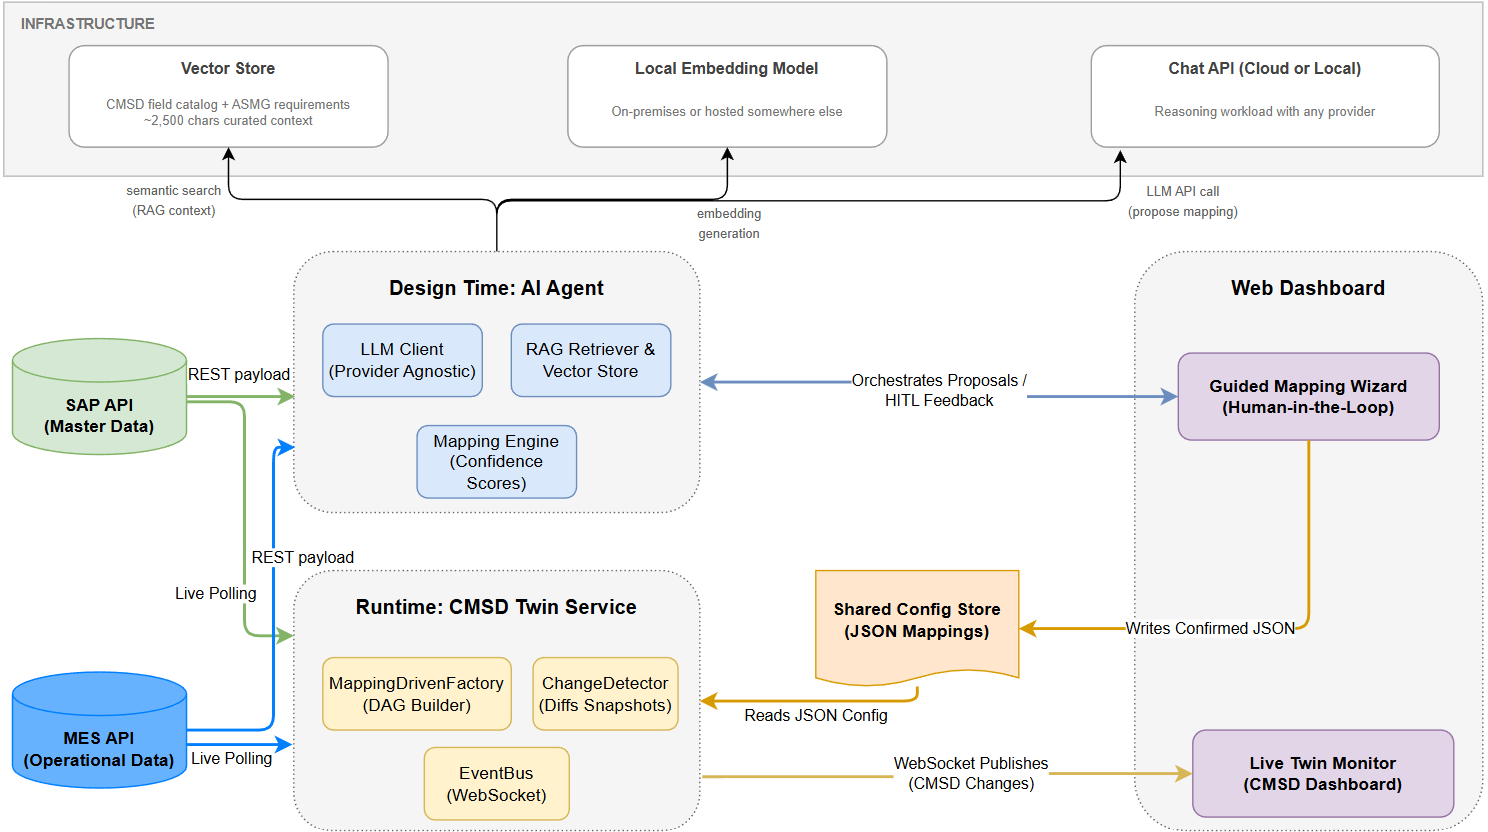
\includegraphics[width=0.75\textwidth]{architecture.png}
\caption{System architecture. The AI Agent proposes mappings at design time; the CMSD Twin Service executes them deterministically at runtime. Source adapters abstract enterprise system heterogeneity behind a uniform fetch interface.}
\label{fig:architecture}
\end{figure}

\subsection{Mapping as Configuration}
\label{sec:arch-config}

The central idea of the architecture is that field mapping between enterprise APIs and a canonical information model is a configuration problem, not a code generation problem. The traditional pattern hard-codes per-field extraction logic: a developer writes conditional branches for each customer and each API variant (e.g., \texttt{if customer == "AcmeCorp": resource.availability = payload["uptime\_pct"] / 100}). The code is opaque to domain experts, brittle under API changes, and rewritten for every new data source. The configuration-driven approach replaces this with a JSON entry: \texttt{\{"api\_path": "uptime\_pct", "transformation": \{"type": "divide\_by", "params": \{"divisor": 100\}\}, "confidence": "high"\}}. A generic MappingDrivenFactory reads this configuration and produces typed CMSD instances at runtime, with no generated code in the execution path.

The JSON configuration is the single source of truth for every mapping decision. It is human-readable, diffable, version-controllable, and language-agnostic. A factory manager can review which API fields map to which CMSD attributes without reading Python. A consultant can version a mapping file alongside the factory's configuration repository. A new customer with different API structures requires only a new JSON file; the engine, the dashboard, and the deployment stack remain unchanged.

\subsection{The Canonical Information Model}
\label{sec:arch-hub}

Enterprise source systems speak different dialects for the same underlying manufacturing concepts. A resource's uptime percentage might appear as \texttt{uptime\_pct} in SAP, \texttt{AVAIL\_PCT} in one MES, and \texttt{availability\_percent} in another. The architecture resolves this by designating a vendor-neutral canonical information model as the integration hub. We use CMSD (Core Manufacturing Simulation Data, ISO~22400) as the reference implementation, but the architecture is schema-agnostic: the same engine, configuration format, and workflow apply to any target model, including AutomationML (AML), the Asset Administration Shell (AAS), or a proprietary schema. The AI layer translates each source dialect into the canonical vocabulary. The twin only knows the canonical model, so source heterogeneity is fully abstracted. Swapping the target schema requires only a different field catalog in the RAG store and a different set of typed model implementations in the factory; the mapping pipeline and runtime engine remain unchanged.

\subsection{Multi-Endpoint Data Fusion}
\label{sec:arch-fusion}

A single digital twin entity often requires data from multiple independent APIs. A Resource entity, for instance, draws its static attributes from SAP (name, capacity, type, location), its live operational state from one MES endpoint (busy, idle, offline), and its reliability metrics from another (MTTR, MTBF, failure count). The architecture performs concurrent fetch across all source endpoints, with each endpoint succeeding or failing independently. The twin is assembled from whichever data arrives; a failed endpoint does not block the others. Every mapped field records its source attribution (which API, which endpoint, which join key), enabling traceability from CMSD instance back to the originating system. Cross-endpoint instance matching uses a declared join key (such as \texttt{resource\_id}) to merge data from multiple APIs into a single CMSD entity.

\subsection{DAG-Driven Entity Construction}
\label{sec:arch-dag}

CMSD entities reference each other. An Order references a PartType through its order lines. A Job references a Resource. A Bill of Materials references Parts. Building these entities in the wrong order breaks referential integrity: an Order that references a PartType identifier that has not yet been generated is structurally invalid.

A MappingRegistry constructs a dependency Directed Acyclic Graph (DAG) from the relationships declared in each mapping configuration, shown in Figure~\ref{fig:dag}. Topological sort determines the correct build order (ResourceClasses, then Resources, then PartTypes, then Orders, then Jobs), ensuring that referenced entities exist before they are referenced. Before any generation begins, a pre-flight validation pass checks three conditions: dependency completeness (every referenced entity type has a selected mapping), field coverage (every field on every selected mapping has been reviewed and approved), and API reachability (each source endpoint responds to a health check). If validation passes, the system guarantees a structurally sound digital twin.

The LLM assists entity relation discovery during the mapping phase. When it detects a field like \texttt{part\_type\_id} in an Order API payload, it proposes a relation to the PartType entity with the corresponding match key. The human operator accepts, edits, or rejects each proposed relation. The DAG is built from approved relations, not inferred at runtime.

\begin{figure}[t]
\centering
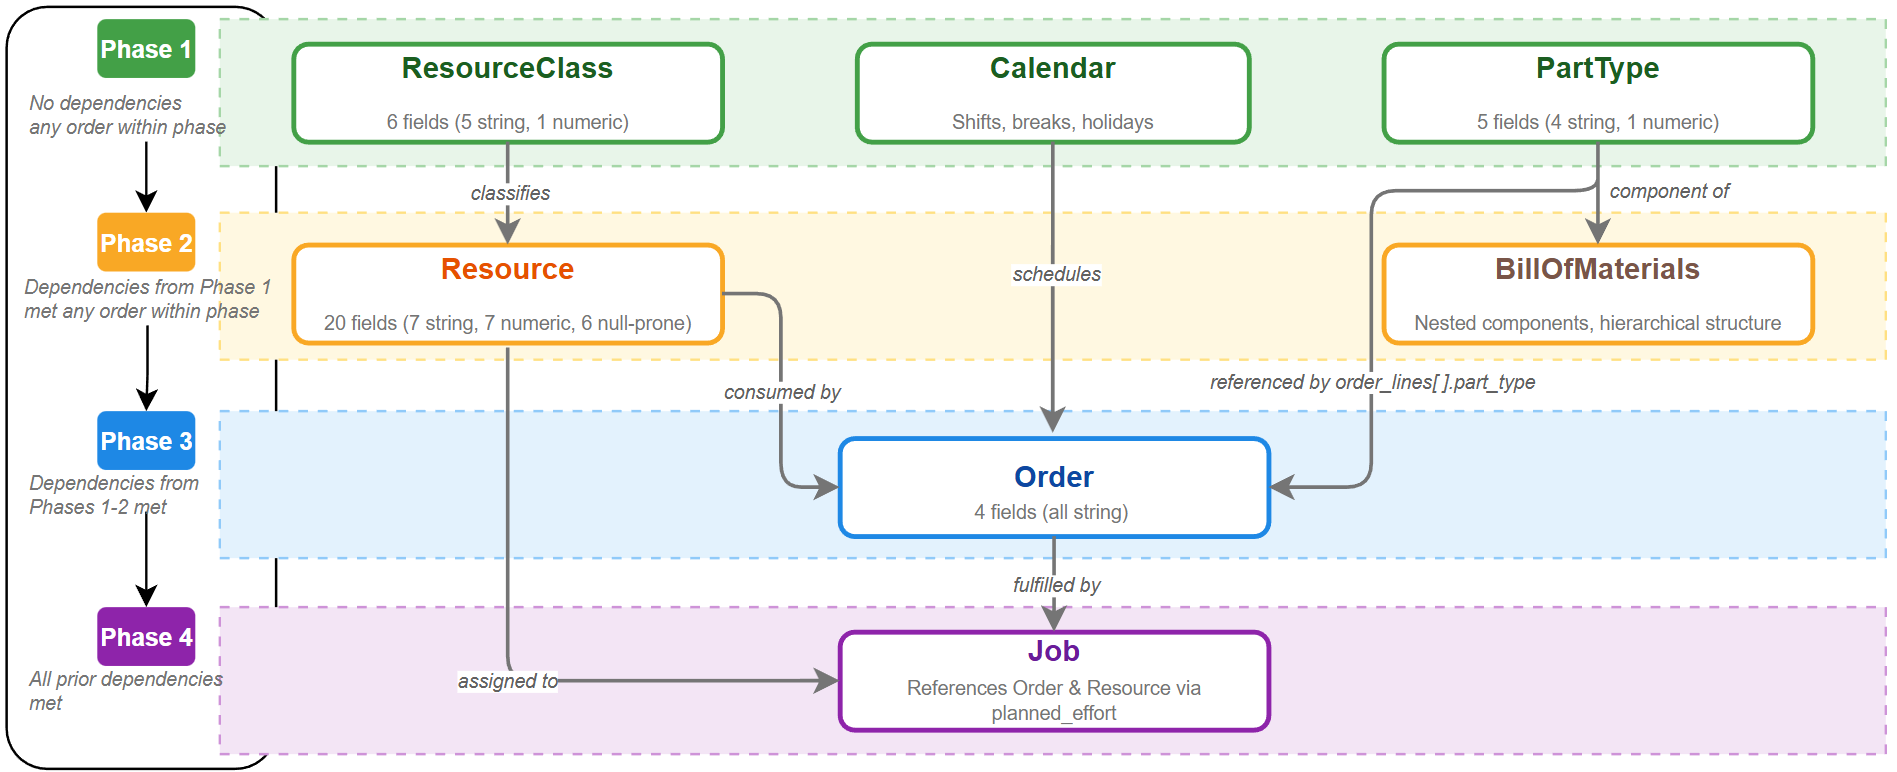
\includegraphics[width=0.7\textwidth]{ISM2026_dag.png}
\caption{Entity dependency DAG. Topological sort determines the correct build order, ensuring referential integrity across the assembled digital twin.}
\label{fig:dag}
\end{figure}

\subsection{Human-in-the-Loop with Calibrated Confidence}
\label{sec:arch-hitl}

The guided mapping workflow proceeds through six phases: Connect (select source systems and enter endpoint paths), Approve (review fetched payloads, exclude failed endpoints), Map (LLM proposes field-level mappings with RAG context), Review (human inspects proposals flagged as uncertain), Transform (human selects and previews conversion rules), and Generate (configuration is saved and the twin is assembled). Each phase constrains the next; the wizard enforces the workflow so the user does not need to understand it in advance.

The LLM self-scores every mapping proposal as high, medium, or low confidence. High-confidence proposals are collapsed by default in the review interface and are safe to auto-accept. Medium and low-confidence proposals are surfaced for mandatory human inspection. When a human corrects a flagged field, the system performs smart reanalysis: it re-evaluates only the corrected field against the updated constraint, leaving all previously accepted mappings intact. This targets human effort exclusively where the model is uncertain and prevents a single correction from triggering a full re-mapping.

For the SME operator, this workflow means that CMSD expertise is not a prerequisite. The AI makes the first proposal; the human reviews only what the model flags. Review effort scales with API quality, not entity complexity. Expert corrections are captured in persistent configuration files and compound across factories.

\subsection{Continuous Synchronization}
\label{sec:arch-sync}

The architecture treats the digital twin as a living representation of the factory, not a one-time export. The synchronization cycle follows five stages: poll (on a configurable interval, or triggered manually), fetch (concurrent API calls to all source endpoints), build (MappingDrivenFactory assembles a new CMSD document), diff (ChangeDetector compares the new document against the previous snapshot), and push (EventBus publishes only the changed fields to the dashboard via WebSocket). The default mode is manual refresh; configurable auto-polling can be enabled for continuous operation.

\subsection{Design Rationale for AI-Enabled Manufacturing}
\label{sec:arch-rationale}

Three manufacturing-specific concerns motivated key architectural choices.

\textit{Why deterministic runtime matters.} A shop floor cannot tolerate LLM hallucinations or API latency in its production data path. The LLM operates at design time, proposing mappings during initial configuration and during periodic reconfiguration when APIs change. The production path (fetch APIs, extract fields, apply transforms, build instances, diff, publish) is pure deterministic code. This eliminates unpredictability, variable latency, and per-call cost from the critical runtime.

\textit{Why JSON over code generation.} A JSON mapping file can be read, reviewed, and signed off by a factory manager who understands manufacturing concepts but not programming. The configuration serves as both executable specification and living documentation of every mapping decision. Version-controlling a JSON file alongside the factory's configuration repository gives the mapping the same audit trail as any other operational asset.

\textit{Why open-source models running locally.} Manufacturing data (resource configurations, production orders, operational metrics) is commercially sensitive and, in regulated industries, subject to data residency requirements. The architecture provides possibility to connect to embedding models and chat models running locally, keeping enterprise data on-premises throughout the RAG indexing and retrieval pipeline.

% =============================================================================
% 4. AI-POWERED MAPPING PIPELINE
% =============================================================================
\section{AI-Powered Mapping Pipeline}
\label{sec:pipeline}

% ---------------------------------------------------------------------------
% 4.1 RAG with Curated CMSD Content
\subsection{RAG with Curated Content}
\label{sec:pipeline-rag}

The RAG pipeline retrieves semantic descriptions of CMSD target fields to ground the LLM’s mapping proposals. A ChromaDB vector store indexes two document collections: a curated CMSD field catalog (entity name, field name, type, and plain-English description for every attribute) and a data requirements specification extracted with VDI 3633 Part 1 specification [Reference needed]. Document chunks are embedded using openly available embedding model ( locally run qwen3-embedding:4b, producing 2,560-dimensional vectors for this implementation) and retrieved via cosine similarity. The top-$k$ results are assembled into a compact context window of approximately 2,500 characters and injected into the LLM prompt alongside the source API payload and the system instructions.

The catalog format is deliberately not source code. It contains no type annotations, no Optional wrappers, no Pydantic class definitions. Each entry is a four-field reference row: entity, field, type, and description. We experimentally confirmed that raw source-code retrieval degrades mapping accuracy compared to a clean catalog: the LLM was distracted by implementation-level detail that carries no semantic value for the field-mapping task. Section~\ref{sec:evaluation} quantifies this effect.

A deliberate architectural choice limits RAG to target-side content only. The CMSD schema is fixed and invariant across all deployments. The source API schemas vary per factory, some are well-documented, many legacy systems have no field-level documentation at all. Embedding source-side descriptions would make mapping accuracy dependent on per-customer documentation quality. Our evaluation therefore tests the worst case: what happens when the LLM has target-side context but zero source-side field documentation. The catalog describes what the CMSD field \texttt{availability} means; it does not describe what the source field \texttt{FLD007} represents.

% ---------------------------------------------------------------------------
% 4.2 Provider-Agnostic Multi-Model Support
\subsection{Provider-Agnostic Multi-Model Support}
\label{sec:pipeline-models}

A single LLMClient abstraction wraps any OpenAI-compatible API, allowing the chat model to be swapped by changing environment variable and credentials. The chat provider (cloud or locally hosted LLM) and the embedding provider (local or also cloud) are configured independently. Our evaluation compares two configurations of the same model family: deepseek-v4-flash (reasoning-disabled variant) and deepseek-v4-pro (a reasoning variant). The non-reasoning model was selected to assess whether lightweight inference can match heavyweight reasoning for structured schema mapping, and to validate a deployment path that an SME can replicate with openly available model weights for full data sovereignty.

% =============================================================================
% 5. EVALUATION
% =============================================================================
\section{Evaluation}
\label{sec:evaluation}

\subsection{Experimental Setup}
\label{sec:eval-setup}

The evaluation tests the mapping pipeline across four independent variables. Four API payload variants represent different surface representations of the same underlying manufacturing data: \texttt{clean} (well-named English fields, the baseline), \texttt{legacy} (all field names replaced with opaque codes FLD001 through FLD201, simulating undocumented legacy systems), \texttt{german} (all field names in German, representing DACH-region manufacturing deployments), and \texttt{deep} (data wrapped in a three-level JSON envelope, testing nested-response navigation). Four CMSD entity types of varying complexity were selected: Resource (20 fields: 7 string, 7 numeric, 6 null-prone), ResourceClass (6 fields: 5 string, 1 numeric), Order (4 string fields), and PartType (5 fields: 4 string, 1 numeric). Two LLM configurations were tested: deepseek-v4-flash (reasoning disabled) and deepseek-v4-pro (reasoning enabled). Two RAG conditions were ablated: no retrieval at all, and catalog RAG. Ground truth mappings were defined per variant per entity and manually verified field by field. All experiments are reproducible via a test harness script.

The primary metric is mapping accuracy: the percentage of ground-truth fields correctly assigned to their CMSD targets. Secondary metrics include string-field accuracy, numeric-field accuracy, prompt tokens, completion tokens, total tokens, and latency per entity.

The experimental design uses a two-phase strategy. Phase I establishes baselines with $n = 5$ runs across both models, all four entities, all four variants, and both RAG modes. Phase II executes an extended longitudinal probe ($n = 20$) on the Flash model only, toggling RAG on and off, yielding 640 total runs. This expanded dataset enables robust non-parametric statistical testing (Mann--Whitney $U$ and Levene's test) to determine whether RAG provides statistically significant improvement in mapping accuracy or output consistency.


% ---------------------------------------------------------------------------
% 5.2 Accuracy Results
% ---------------------------------------------------------------------------
\subsection{Accuracy Results}
\label{sec:eval-accuracy}

Table~\ref{tab:aggregate-accuracy} reports aggregate mapping accuracy by model and RAG mode across all entities and variants. Both models achieve 95--96\% aggregate accuracy. The non-reasoning Flash model matches the reasoning Pro model within 1.4 percentage points while running 2--3$\times$ faster. Pro with catalog RAG achieves perfect string-field accuracy (100.0\%), meaning no string-typed field was ever misassigned with retrieval-augmented context.

\begin{table}[h]
\caption{Aggregate mapping accuracy by model and RAG mode ($n=5$, single-instance).}
\label{tab:aggregate-accuracy}
\begin{tabular*}{\hsize}{@{\extracolsep{\fill}}lcccc@{}}
\toprule
Model & No-RAG & Catalog RAG & String Acc.\ (RAG) & Numeric Acc.\ (RAG) \\
\colrule
deepseek-v4-flash & 95.8\% & 95.0\% & 99.3\% & 93.6\% \\
deepseek-v4-pro  & 95.8\% & 96.4\% & 100.0\% & 95.2\% \\
\botrule
\end{tabular*}
\end{table}

The modest RAG delta on aggregate masks a critical asymmetry that emerges at the per-entity level. Three of four entity types perform at or near ceiling: Order achieves 100\% accuracy across all 16 configurations (4 variants $\times$ 2 RAG modes $\times$ 2 models), reflecting its composition of four string-typed fields with zero numeric and zero null-prone fields. ResourceClass and PartType reach 96--100\% across all variants. Resource is the sole bottleneck: its 20 fields include seven numeric fields and six null-prone fields, and it posts the lowest accuracy in every experimental configuration. Resource's underperformance is not a function of size but of composition. Six of its fields can be null, providing zero identity signal when empty, and its seven numeric fields carry values that lack the semantic cues present in string data. Table~\ref{tab:entity-profiles} shows the field-type composition of each entity. Difficulty correlates with numeric field count and null-proneness, not with total field count.

\begin{table}[h]
\footnotesize
\caption{Entity field type profiles. Difficulty is driven by numeric count and null-proneness, not total fields.}
\label{tab:entity-profiles}
\begin{tabular*}{\hsize}{@{\extracolsep{\fill}}lccccc@{}}
\toprule
Entity & String & Numeric & Null-prone & Total & Difficulty \\
\colrule
Resource      & 7 & 7 & 6 & 20 & Hard (numeric + nulls) \\
ResourceClass & 5 & 1 & 0 &  6 & Moderate \\
Order         & 4 & 0 & 0 &  4 & Easy \\
PartType      & 4 & 1 & 0 &  5 & Easy \\
\botrule
\end{tabular*}
\end{table}

% ---------------------------------------------------------------------------
% 5.3 Evaluating the Contribution of RAG Context
% ---------------------------------------------------------------------------
\subsection{Evaluating the Contribution of RAG Context}
\label{sec:eval-statistical}

RAG with target-side content added approximately 35\% to prompt tokens while increasing completion tokens by only 8\%, localizing its cost to the input phase. Given that Flash achieves Pro-comparable accuracy at lower cost, and that RAG's aggregate benefit was both modest and statistically inconclusive after Phase I, Flash was the natural choice for an extended statistical probe: if RAG cannot meaningfully improve the faster, cheaper model on the hardest mapping cases, then deploying it adds only token overhead without resolving the underlying ambiguity. Phase II executed this probe with $n = 20$ runs per configuration on Flash, yielding 320 runs with RAG and 320 runs without, across all entity-variant pairs. Table~\ref{tab:statistical} reports the results.

\begin{table}[h]
\footnotesize
\caption{RAG vs.\ no-RAG extended statistical analysis (Flash, $n=20$, 640 total runs). Mann--Whitney $U$ test; all $p > 0.05$. Ranges shown in brackets.}
\label{tab:statistical}
\begin{tabular*}{\hsize}{@{\extracolsep{\fill}}llccc@{}}
\toprule
Entity & Variant & RAG Median [Min, Max] & No-RAG Median [Min, Max] & $p$ (MWU) \\
\colrule
Resource      & legacy        & 45.0\% [30.0, 65.0]  & 45.0\% [35.0, 60.0]  & 0.657 \\
Resource      & clean         & 100.0\% [65.0, 100.0] & 100.0\% [65.0, 100.0] & 0.986 \\
Resource      & german        & 100.0\% [70.0, 100.0] & 100.0\% [70.0, 100.0] & 0.252 \\
Resource      & deep          & 100.0\% [95.0, 100.0] & 100.0\% [95.0, 100.0] & 0.225 \\
PartType      & clean/german  & 100.0\% [80.0, 100.0] & 100.0\% [80.0, 100.0] & $\geq$0.654 \\
ResourceClass & legacy/german & 100.0\% [83.3, 100.0] & 100.0\% [83.3, 100.0] & $\geq$0.302 \\
Order         & all variants  & 100.0\% [100.0, 100.0] & 100.0\% [100.0, 100.0] & 1.000 \\
\botrule
\end{tabular*}
\end{table}

Across all 640 runs, the Mann--Whitney $U$ test yields $p > 0.05$ for every entity-variant pair. RAG provides zero statistically significant improvement to mapping accuracy. Levene’s test for equality of variances ($p = 0.9631$) further confirms that RAG does not stabilize output consistency: the model is equally volatile with or without retrieval. Resource legacy is the catastrophic case (median 45\%, range 30--65\%, $p = 0.657$). Order is the ideal case (deterministic 100\%, $p = 1.000$), with or without RAG.

The failure mode is not a retrieval quality problem; it is a data problem. String values carry identity cues: ``CNC Machine 3000’’ reads as a name, ``ACTIVE’’ reads as a status. Numeric values carry no such signal: 95.0 could be availability (as a percentage), efficiency, hourly rate, or machine count. When the LLM encounters \texttt{FLD007: 95.0} alongside seven numeric CMSD fields all within the 0--100 range, the catalog narrows the target-side range (availability must be a 0.0--1.0 fraction, so 95.0 cannot be a raw availability value) but cannot disambiguate among the remaining candidates. This is aleatoric ambiguity inherent to the source data, not epistemic uncertainty that better retrieval could resolve. The cross-model data confirms this is model-agnostic: Pro achieves only 46--50\% on the same Resource-legacy bottleneck, with the additional handicap of a 60\% timeout rate on the hardest variant. Pro's deeper reasoning produced per-entity latencies exceeding 180 s in 3 of 5 runs for those variants, a regime where the speed advantage of automation narrows. Neither retrieval quality nor model scaling compensates for structural ambiguity in the source payload.

% ---------------------------------------------------------------------------
% 5.4 Confidence Calibration
% ---------------------------------------------------------------------------
\subsection{Confidence Calibration}
\label{sec:eval-confidence}

The LLM's self-assessed confidence scores align with empirical accuracy. High-confidence proposals are correct in over 95\% of cases across both models, validating the architecture's claim that high-confidence fields are safe to auto-accept. Medium and low-confidence proposals consistently correspond to the fields that are empirically incorrect, particularly on legacy cryptic payloads where the LLM correctly recognizes its own uncertainty. The system does not assert false certainty on hard cases: incorrect legacy numeric-field mappings consistently receive medium or low confidence scores. This calibration is what makes the human-in-the-loop workflow viable: the human operator reviews only the subset of fields the model itself flags, rather than exhaustively verifying every proposal.

% =============================================================================
% 6. DISCUSSION
% =============================================================================
\section{Discussion}
\label{sec:discussion}

The evaluation results delineate clear boundaries for where the system delivers fully automated mapping and where human intervention remains necessary. When source APIs use well-named fields and target entities are well-typed, the system achieves 100\% accuracy with either model, with or without RAG. This includes entities with deeply nested JSON payloads, where the LLM correctly navigates multi-level nesting to extract leaf values, and entities with non-English field names, where accuracy remains at 96--100\% across all tested variants. Notably, string-only entities perform at 100\% even on legacy cryptic payloads: when all four fields of an Order carry semantically rich string values, the LLM infers field identity from value content alone and never misassigns a field.

The fundamental bottleneck is numeric ambiguity. On the Resource entity's legacy variant, where seven numeric fields are identified only by opaque FLD codes within overlapping 0--100 ranges, accuracy drops to 41--50\% regardless of model or RAG. The catalog provides target-side semantic constraints (availability must be a 0.0--1.0 fraction) but cannot resolve which opaque numeric field maps to which CMSD attribute when the values themselves carry no distinguishing signal. Null-valued fields compound the problem: six of Resource's 20 fields can be null, and a null value provides zero information about field identity. This is not a retrieval quality issue; it is a fundamental information asymmetry between string and numeric data that no amount of target-side context can resolve.

For the SME operator, the practical implications are encouraging. The system requires no CMSD expertise to begin. The AI proposes; the human reviews only what the model flags. Effort scales with source API quality, not entity complexity. For modern, well-documented APIs, the system can operate without RAG at 95.8\% accuracy, with lower latency and simpler infrastructure. Configurations persists as expert corrections are captured once and reused across factories, and the same JSON file that maps one factory's SAP instance can serve as the starting point for another.

The durable contribution of this work is the architecture itself. The JSON configuration decouples AI-driven proposal from deterministic execution and the design-time/runtime separation guarantees production safety regardless of LLM behavior.

\section{Conclusion}
\label{sec:conclusion}

We presented a human-in-the-loop architecture for LLM-driven digital twin assembly from heterogeneous enterprise APIs. The core innovation is treating field mapping as a configuration problem rather than a code generation problem and a vendor-neutral canonical information model abstracts away all source-system heterogeneity.

Both evaluated LLM configurations achieve 95--96\% aggregate mapping accuracy. A non-reasoning model matches reasoning-model accuracy within 1.4 percentage points while running 2--3$\times$ faster with lower token consumption. Extended statistical analysis ($n = 20$, 640 runs) establishes that numeric field ambiguity in legacy payloads is the fundamental bottleneck: target-side RAG provides zero statistically significant improvement (Mann--Whitney $U$, $p > 0.05$).

Future work proceeds along three directions. The primary extension is graph-native digital twin instances with built-in reasoning for automatic relation propagation, blast-radius analysis, and schema-change cascade management, extending the architecture from instance assembly to instance lifecycle management. Second, production deployment with live enterprise connectors will validate the architecture against the complexities of real manufacturing IT environments. Third, a controlled user study with manufacturing SMEs will quantify the reduction in time-to-twin and review burden that the calibrated confidence workflow enables in practice.

This work demonstrates that thoughtful software architecture, not just model capability, is the key to making AI useful in manufacturing. The LLM provides flexibility and the deterministic engine provides reliability while the JSON configuration bridges them. For the thousands of SMEs that cannot afford embedded software consultants, this architecture offers a path to industrial-grade digital twins that was previously closed.

% =============================================================================
% ACKNOWLEDGEMENTS
% =============================================================================
%\section*{Acknowledgements}
% TODO

% =============================================================================
% REFERENCES
% =============================================================================
\bibliographystyle{elsarticle-num-names}
\bibliography{references}

\end{document}
